% Options for packages loaded elsewhere
\PassOptionsToPackage{unicode}{hyperref}
\PassOptionsToPackage{hyphens}{url}
%
\documentclass[
]{book}
\usepackage{amsmath,amssymb}
\usepackage{lmodern}
\usepackage{ifxetex,ifluatex}
\ifnum 0\ifxetex 1\fi\ifluatex 1\fi=0 % if pdftex
  \usepackage[T1]{fontenc}
  \usepackage[utf8]{inputenc}
  \usepackage{textcomp} % provide euro and other symbols
\else % if luatex or xetex
  \usepackage{unicode-math}
  \defaultfontfeatures{Scale=MatchLowercase}
  \defaultfontfeatures[\rmfamily]{Ligatures=TeX,Scale=1}
\fi
% Use upquote if available, for straight quotes in verbatim environments
\IfFileExists{upquote.sty}{\usepackage{upquote}}{}
\IfFileExists{microtype.sty}{% use microtype if available
  \usepackage[]{microtype}
  \UseMicrotypeSet[protrusion]{basicmath} % disable protrusion for tt fonts
}{}
\makeatletter
\@ifundefined{KOMAClassName}{% if non-KOMA class
  \IfFileExists{parskip.sty}{%
    \usepackage{parskip}
  }{% else
    \setlength{\parindent}{0pt}
    \setlength{\parskip}{6pt plus 2pt minus 1pt}}
}{% if KOMA class
  \KOMAoptions{parskip=half}}
\makeatother
\usepackage{xcolor}
\IfFileExists{xurl.sty}{\usepackage{xurl}}{} % add URL line breaks if available
\IfFileExists{bookmark.sty}{\usepackage{bookmark}}{\usepackage{hyperref}}
\hypersetup{
  pdftitle={Technology},
  pdfauthor={Dyrehaugen Web Notebook},
  hidelinks,
  pdfcreator={LaTeX via pandoc}}
\urlstyle{same} % disable monospaced font for URLs
\usepackage{longtable,booktabs,array}
\usepackage{calc} % for calculating minipage widths
% Correct order of tables after \paragraph or \subparagraph
\usepackage{etoolbox}
\makeatletter
\patchcmd\longtable{\par}{\if@noskipsec\mbox{}\fi\par}{}{}
\makeatother
% Allow footnotes in longtable head/foot
\IfFileExists{footnotehyper.sty}{\usepackage{footnotehyper}}{\usepackage{footnote}}
\makesavenoteenv{longtable}
\usepackage{graphicx}
\makeatletter
\def\maxwidth{\ifdim\Gin@nat@width>\linewidth\linewidth\else\Gin@nat@width\fi}
\def\maxheight{\ifdim\Gin@nat@height>\textheight\textheight\else\Gin@nat@height\fi}
\makeatother
% Scale images if necessary, so that they will not overflow the page
% margins by default, and it is still possible to overwrite the defaults
% using explicit options in \includegraphics[width, height, ...]{}
\setkeys{Gin}{width=\maxwidth,height=\maxheight,keepaspectratio}
% Set default figure placement to htbp
\makeatletter
\def\fps@figure{htbp}
\makeatother
\setlength{\emergencystretch}{3em} % prevent overfull lines
\providecommand{\tightlist}{%
  \setlength{\itemsep}{0pt}\setlength{\parskip}{0pt}}
\setcounter{secnumdepth}{5}
\usepackage{booktabs}
\usepackage{amsthm}
\makeatletter
\def\thm@space@setup{%
  \thm@preskip=8pt plus 2pt minus 4pt
  \thm@postskip=\thm@preskip
}
\makeatother

\renewcommand\chaptername{}
\ifluatex
  \usepackage{selnolig}  % disable illegal ligatures
\fi
\usepackage[]{natbib}
\bibliographystyle{apalike}

\title{Technology}
\author{Dyrehaugen Web Notebook}
\date{2021-05-03}

\begin{document}
\maketitle

{
\setcounter{tocdepth}{1}
\tableofcontents
}
\hypertarget{technology}{%
\chapter{Technology}\label{technology}}


\includegraphics{fig/zelda.jpg}

\hypertarget{concrete}{%
\chapter{Concrete}\label{concrete}}

We live in a world of concrete. After water, it's the most widely used substance on our planet, and its usage around the world, ton for ton, is twice that of steel, wood, plastics and aluminium combined.

Its invention in 1824, by a bricklayer in Leeds who first produced the Portland cement used to bind the aggregates used in concrete, quite literally paved the way for the creation of the modern world, enabling humans to mould high-strength, stone-like structures of almost any shape.

Concrete's ubiquity comes at a high price though: if the cement industry were a country, it would be the third-largest emitter of carbon dioxide in the world, after the US and China, as it releases over 2.8 billion tonnes into the atmosphere each year.

A 2018 report suggested concrete contributes up to 8 per cent of the world's CO2 emissions.

It also requires phenomenal amounts of water, sucking up around a tenth of all water used in industry -- often in areas with critical water shortages.

\href{https://www.independent.co.uk/climate-change/news/wood-construction-concrete-steel-climate-b1796342.html}{Cockburn}

\hypertarget{steel}{%
\chapter{Steel}\label{steel}}

Today, the U.S. only accounts for about 5 percent of global steel production capacity.

If the U.S. is to achieve Biden's vision of a new deal for America, complete with infrastructure upgrades, domestically sourced materials and net-zero emissions, the country needs not only to reverse its flagging fortunes in the steel market but also to foster new technologies that will enable it to produce ``green'' steel with a minimum of carbon dioxide emissions. Such new technologies are now under development, although their entry into the marketplace is going to require time, investment and government support.

Steel production is one of humanity's most environmentally destructive activities. Even in its diminished state, the U.S. steel industry releases more carbon dioxide emissions than any other domestic industry --- nearly a ton of carbon dioxide for every ton of steel produced.

That's largely because steel-making relies on coal and natural gas for most of its hefty energy consumption.

Steel industry emissions must be mitigated at first by eking out small improvements to a wide variety of production stages. Simply using steel more efficiently is the first step. For example,
some \href{https://energycentral.com/c/ec/new-innovation-drives-down-carbon-dioxide-emissions-cement}{new forms of concrete} are structurally stable without the use of steel reinforcing bars. Also, other materials can be substituted for steel;
one young company called \href{https://www.inventwood.com/}{Inventwood} is developing a process that transforms wood into \href{https://www.inventwood.com/mettlewood/}{a material strong enough to be used in place of steel}.

Another technique is to recycle more steel. According to the International Energy Agency, producing steel from recycled scrap requires only one-eighth the energy associated with producing steel from iron ore. Scrap accounts for about 70 percent of the raw metal input to U.S. steel production today, a figure that can be boosted.

But that alone won't obviate the need for new steel mills, since future demand for steel will outpace past supply. Instead, the U.S. will have to make new steel from iron ore and mitigate the emissions stemming from that process.

To better understand the options for improvement, let's review how steel is typically made. First, iron ore and fossil fuels (usually either specially refined coal or natural gas) are put in a furnace, where the fuels are burned to produce heat, carbon monoxide and carbon dioxide. The carbon monoxide combines with oxygen from the iron oxide contained in the ore, forming carbon dioxide and leaving behind a quantity of nearly pure iron. That iron is then conveyed either to a specially lined vat where oxygen is blown through liquid iron or to an electric furnace. In these secondary vessels, the iron is further purified and combined with small amounts of carbon to make steel.

One way to mitigate the carbon emissions from this process is to capture carbon dioxide from the furnace and sequester it in underground reservoirs.
Most carbon-capture facilities don't actually sequester the carbon dioxide they capture. Instead, they sell it to oil companies that then pump it underground to force oil to the surface, a process known as enhanced oil recovery (EOR).
The only operating steel plant using carbon capture at scale, the Al Reyadah plant in Abu Dhabi, employs this technique.
It's not clear that EOR sequestration actually reduces emissions on a net basis if the calculation includes the carbon dioxide released by burning the oil that's produced.
It's unlikely this technique will result in significant reductions of net emissions.

Other techniques include improving the efficiency of the ore processing furnaces and replacing coal furnaces with natural-gas furnaces. These techniques will only provide marginal emission reductions.

\textbf{New steel-making technologies}

\textbf{\emph{H2 DRI}}

The two leading steel-making technologies with the potential to nearly eliminate carbon dioxide emissions use a common chemical process known as electrolysis.

One technology that's well on its way is called ``hydrogen direct reduced iron'' (H2 DRI). It is now being demonstrated in Sweden, Japan and Germany. H2 DRI substitutes hydrogen (preferably, but not necessarily, made with clean energy) for the coal or natural gas used in the typical furnace process. In a DRI furnace, the iron ore is heated but not to the point of melting. Hydrogen then passes over the hot ore, combining with oxygen liberated from the iron oxide to form water and leaving relatively pure iron behind. Typically, that still-hot iron is then transferred to an electric furnace for additional processing to turn it into steel. If the electricity used to produce the hydrogen and run the furnace comes from non-carbon-emitting sources, then the overall process results in little to no carbon dioxide emissions.

In Sweden, a joint venture dubbed Hybrit (comprising utility Vattenfall, iron ore processor LKAB and steel maker SSAB) is running a pilot H2 DRI plant. This spring, it started to use hydrogen produced via electrolysis from electricity generated by fossil-free sources. (This being Sweden, those probably consist of nuclear and hydropower, with a bit of wind power sprinkled in.) Building a full-scale H2 DRI plant, including electrolyzers to produce hydrogen from clean electricity, costs billions of dollars, and the process consumes prodigious amounts of electricity. Its economics strongly depend on the cost of that electricity and the value of the avoided carbon dioxide emissions. According to the consultancy McKinsey, H2 DRI is not expected to be cost-effective in Europe until sometime between 2030 and 2040.

\textbf{\emph{MOE}}

The other technology under development, molten oxide electrolysis (MOE), also employs electrolysis. But in this case, it's applied directly to the iron oxide ore by placing it in an electrolytic cell filled with a mineral-bearing solution. An electric current is run through the solution, heating it up beyond the melting point of iron, and separating oxygen from iron. If the electricity used to power the MOE process comes from clean sources, the steel can be made with virtually no carbon dioxide emissions.

In the U.S., MOE is being developed by Boston Metal, a company spun out of the Massachusetts Institute of Technology. Like H2 DRI, MOE economics are heavily dependent on the cost of clean electricity. Boston Metal is currently gearing up to build its first pilot plant in Massachusetts, and it is looking into building a larger facility in Quebec or another location with cheap hydroelectricity.

\emph{Prospects}

Of the two technologies, H2 DRI is clearly further along, with a pilot plant in operation and a full-scale plant in development. MOE has some intriguing advantages for the U.S. market, however. First, it's more efficient, requiring somewhere between 15 and 30 percent less electricity than H2 DRI per ton of steel output. Second, MOE facilities can be constructed in much smaller increments than H2 DRI, although exactly how small isn't clear just yet. That's a big deal in the U.S., where a diminished steel industry is unlikely to invest billions of dollars for a new steel plant based on new technology.

Furthermore, Boston Metal's electrolysis cells are so clean that developers would have far more flexibility in where they're located. For example, they could be placed near inexpensive sources of clean electricity or iron ore, or maybe even in Pittsburgh. Both technologies are going to take at least a decade before they're ready to start claiming significant amounts of market share, but over the long run, the odds of Boston Metal's MOE technology gaining traction in the U.S. market appear to be better.

Because steel constitutes just a small portion of most products of which it's a component, that price premium is likely to be small. For example, the International Energy Agency estimates that using green steel would increase the cost of a midsized car by around 0.1\%

\href{https://www.canarymedia.com/articles/joe-bidens-green-new-steel/}{CanaryMedia}

\hypertarget{wood}{%
\chapter{Wood}\label{wood}}

Architects and developers are increasingly aware of the role played by steel and concrete manufacturing in the worsening climate crisis, and there is already a move in some quarters towards much more sustainable building materials.

One such material is already being widely used in construction, but recent advances mean it is stronger and more durable than it has ever been before, and has a far, far lower environmental impact than concrete or steel. That material is wood.

Though timber-framed buildings are hardly new, instead of sawing enormous beams from ancient trees, new techniques focus on using fast-growing soft woods, stuck together in a form which provides massive strength, durability, and flexibility of design.

One example of this, cross-laminated timber (CLT), is manufactured using a technique developed in the 1990s in Austria, in which sheets of kiln-dried wood are glued on top of each other, with the grain of each layer running perpendicular to the next.

This method can create huge boards, up to a foot thick, and as long and as wide as the manufacturer's premises allow.

What's more, the strength of these coagulated timber slabs can match or exceed steel or concrete.

The use of CLT as a modern construction material has already been definitively proven.

The world's largest CLT structure is Dalston Works, a 10-storey residential building of 101 flats, in Hackney, London, which was completed in 2017, and won the ``eco living award'' at the Evening Standard's 2018 New Homes Awards.

Meanwhile, the world's tallest timber building has also been built using CLT -- the 85.4-metre, 18-storey Mjostarnet building in Norway, which was completed in 2019 and is also the country's third-tallest building. The mixed-use building contains apartments, a hotel, a swimming pool, office space and a restaurant.

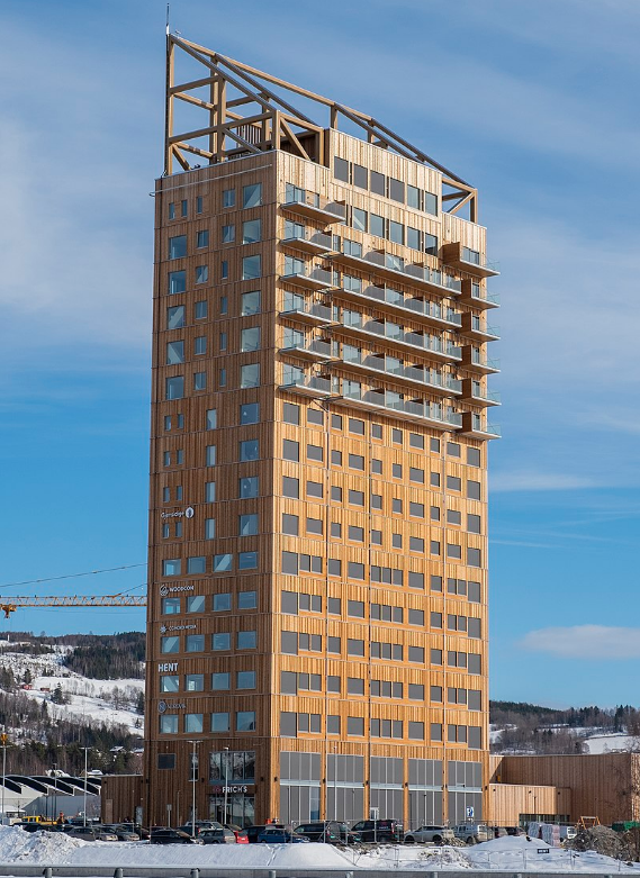
\includegraphics{fig/mjostarnet.png}

\emph{Figure: Mjøstårnet}

For new buildings, the energy regulations are pushing energy consumption and carbon emissions down to the point that the main carbon emissions from new buildings through their life cycle come from their construction and materials.

CLT buildings may be able to store more carbon in the wood than their entire construction generates.

As trees absorb CO2 when they grow, CLT is considered to have a negative embodied carbon -- meaning that the CO2 absorbed by the tree during its growth can be more than that emitted in the manufacture of the CLT product and its transportation to the site.

At the end of its useful life CLT can be repurposed -- something tricky to achieve with other building materials.

The timber used should come from managed forests which have been properly certified as being sustainable sources of wood.

However, ``sustainable forestry'' is a contentious subject, with different meanings in different countries. While vast forests of fast-growing conifers may be able to rapidly fulfil timber orders, a growing understanding of the impact of monoculture cropping on biodiversity, and what it means for carbon sequestration, is also a key consideration for those seeking to herald CLT as a straightforward environmentally friendly choice.

The wood used in the 10-storey Dalston Works building in London was grown in forests in Austria and Germany which have been certified as sustainable.

It was then manufactured into CLT in Austria and brought by road to the UK.

According to the developers, the building used 4,500 cubic metres of timber, which equates to about 2,300 trees. With more than 800 people living in the building, they say it worked out at about three trees per person.

the main tree grown for construction in the UK is the sitka spruce, an imported conifer from the Pacific northwest of North America.

In their home region these trees can reach 40-70 metres in height, but in the UK, where conditions are milder, their growth rate is faster but the resulting density of the wood is lower, making it weaker.

As a result, higher strength timber grown in Europe is normally used for key structural purposes.

One particular concern about the extensive use of wood in construction is the potential for flammability.

In order to be used as a commercial construction material, CLT has been extensively fire-tested, and is designed to accommodate substantial fire resistance.

Furthermore, unlike steel, CLT remains structurally stable when subjected to high temperatures.
CLT is green, cost-effective, fast to install, requires less foundation, and results in less waste than traditional construction.

\emph{From Comments}

It is incorrect to say that CLT ``unlike steel'' remains structurally stable to high temperatures. Steel used in buildings retains at least 100\% of its cold strength up to about 360°°C. (It's actually stronger at around 150-300°C.) What is true is that its insulation properties causes wood to degrade more slowly when exposed to heat as the heat doesn't penetrate so fast. Which is why steam boilers are made out of steel and not wood

\href{https://www.independent.co.uk/climate-change/news/wood-construction-concrete-steel-climate-b1796342.html}{Cockburn}

\hypertarget{part-appendices}{%
\part{Appendices}\label{part-appendices}}

\hypertarget{appendix-appendices}{%
\appendix}


\hypertarget{about}{%
\chapter{About}\label{about}}


\includegraphics{fig/me.jpg}

\emph{Dyre Haugen} and \emph{Dyrehaugen} is Webian for \emph{Jon Martin} -
self-owned Globian, Webian, Norwegian and Canarian with
a background from industrial research policy, urban planning and
economic development consulting on global, regional and urban scales.
I am deeply concerned about the (insane) way
humanity (i.e.~capitalism) interfere with nature.
In an effort to gain insights in how and why this happens
stuff is collected from around the web and put together
in a linked set of web-sites.
The sites are operated as personal notebooks.
However, these days things can be easily published to the
benefit of others concerned with the same issues.
But be aware - this is not polished for presentation or
peer-reviewed for exactness.
I offer you just to have a look at my `work-desk' as it appears in the moment.
Any comment or suggestion can be mailed to \href{mailto:dyrehaugen@gmail.com}{\nolinkurl{dyrehaugen@gmail.com}}
You can follow me on twitter as @dyrehaugen.
Thanks for visiting!

\hypertarget{links}{%
\chapter{Links}\label{links}}

\textbf{Current Dyrehaugen Sites:}

\begin{itemize}
\tightlist
\item
  \href{https://dyrehaugen.github.io/rcap}{rcap - On Capitalism} \href{http://localhost/rcap}{(loc)}
\item
  \href{https://dyrehaugen.github.io/rclm}{rclm - On Climate Change} \href{http://localhost/rclm}{(loc)}
\item
  \href{https://dyrehaugen.github.io/recs}{recs - On Economics} \href{http://localhost/recs}{(loc)}
\item
  \href{https://dyrehaugen.github.io/rngy}{rfin - On Finance} \href{http://localhost/rfin}{(loc)}
\item
  \href{https://dyrehaugen.github.io/rngy}{rngy - On Energy} \href{http://localhost/rngy}{(loc)}
\item
  \href{https://dyrehaugen.github.io/renv}{renv - On Environment} \href{http://localhost/renv}{(loc)}
\item
  \href{https://dyrehaugen.github.io/rsts}{rsts - On Statistics} \href{http://localhost/rsts}{(loc)}
\item
  \href{https://dyrehaugen.github.io/rurb}{rurb - On Urbanization} \href{http://localhost/rurb}{(loc)}
\item
  \href{https://dyrehaugen.github.io/rvar}{rvar - On Varia} \href{http://localhost/rvar}{(loc)}
\item
  \href{https://dyrehaugen.github.io/rwsd}{rwsd - On Wisdom} \href{http://localhost/rwsd}{(loc)}
\end{itemize}

\textbf{Blogs:}

\begin{itemize}
\tightlist
\item
  \href{https://dyrehaugen.github.io/rde}{rde - Blog in English} \href{http://localhost/rde}{(loc)}
\item
  \href{https://dyrehaugen.github.io/rdn}{rdn - Blog in Norwegian} \href{http://localhost/rdn}{(loc)}
\end{itemize}

\textbf{Discontinued:}

\begin{itemize}
\tightlist
\item
  \href{https://dyrehaugen.github.io/jdt}{jdt - Collection (Jekyll)} \href{http://localhost/jdt}{(loc)}
\item
  \href{https://dyrehaugen.github.io/hdt}{hdt - Collection (Hugo)} \href{http://localhost/hdt}{(loc)}
\end{itemize}

\textbf{Not listed:}

\begin{itemize}
\tightlist
\item
  (q:) dhe dhn jrw56
\item
  (z:) rcsa rpad rstart
\end{itemize}

\hypertarget{news}{%
\chapter{NEWS}\label{news}}

  \bibliography{book.bib,packages.bib}

\end{document}
